\chapter{Analis y Dise'no del Servicio Web}
\label{capitulocuatro}

Como se ha mencionado \ref{capitulotres}, para desarrollar el servicio, se debe realizar los detalles del servicio que se desea realizar.
 \section{Analisis del servicio web}
 Para el presente proyecto el analisis se empezara con la descripci'on de servicio que nos ayudara a detallar el servicio con las siguientes documentos:
 \subsection{Documento de interfaz}
 El documento interfaz que responde el \textsl{Que} operaciones soporta el servicio. En el presente proyecto tres procesos:
 \begin{enumerate}
 \item  \textbf{Proceso 1:} primeramente descargan la planilla de notas en el formato .sis, de la p'agina SAGAA, representada en la figura \ref{fig:Proceso1}
 
 \begin{figure}[H]
 \centering
 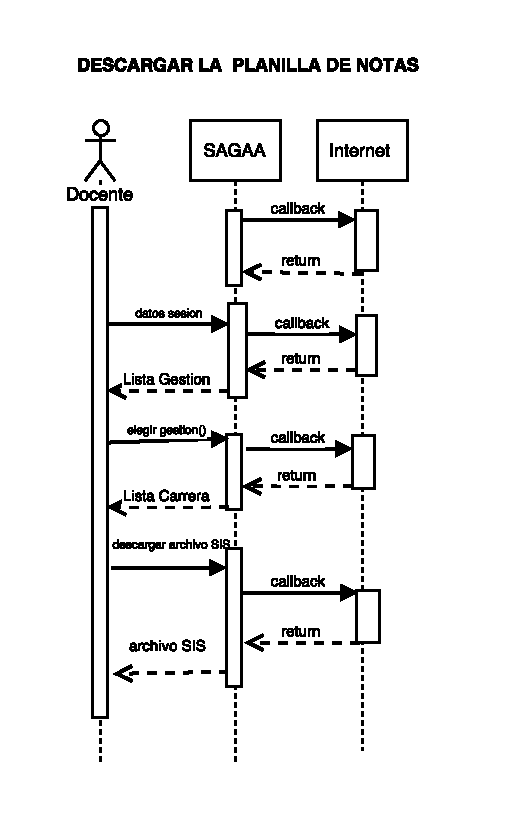
\includegraphics[width=0.3\textwidth]{SdescargarLlenadoNota.pdf}
 \captionsetup{justification=centering,margin=2cm}
 \caption{Proceso de descargar Planilla Notas. Figura: Elaboraci'on propia}
 \label{fig:Proceso1}
 \end{figure}
 
 \item \textbf{Proceso 2:} llenar las notas en la planilla, se utiliza la aplicaci'on del Transcriptor.exe para abrir el documento, representada en la \ref{fig:Proceso2}.
 
 \begin{figure}[H]
 \centering
 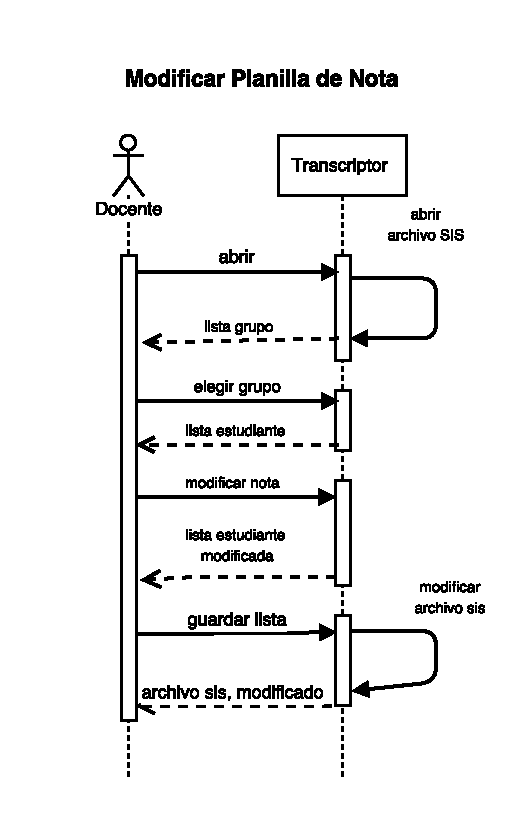
\includegraphics[width=0.3\textwidth]{DSmodificarPlanila.pdf}
 \captionsetup{justification=centering,margin=2cm}
 \caption{Proceso de modificar la Planilla de Notas, Fuente: Elaboraci'on propia}
 \label{fig:Proceso2}
 \end{figure}
   
  \item \textbf{Proceso 3:} para finalizar subimos la planilla de notas, en el formato sis, de la p'agina SAGAA, representada en la \ref{fig:Proceso3}
  
\begin{figure}[H]
\centering
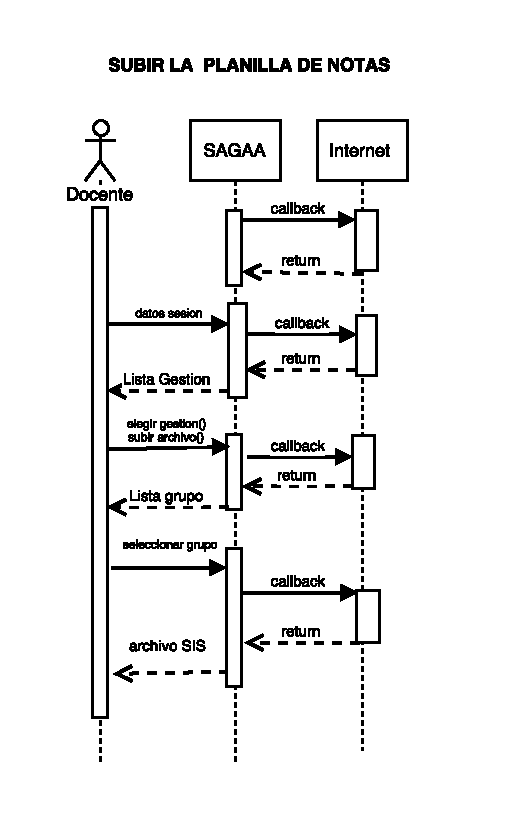
\includegraphics[width=0.3\textwidth]{DSsubirPlanilla.pdf}
\captionsetup{justification=centering, margin=2cm}
\caption{Proceso de subir a la pagina Web SAGAA, Fuente: Elaboraci'on propia}
 \label{fig:Proceso3}
 \end{figure}
 \end{enumerate}

\subsection{Documento enlace}
El documento de enlace que responde el \textsl{C'omo}, es representar graf'icamente la interfaz abstracta a un conjunto concreto de protocolos, que especifica los detalles t'ecnicos de c'omo comunicarse con un servicio.
\begin{figure}
\centering
\includegraphics[width=0.4\textwidth]{comunicacionProtocolo.pdf}
\captionsetup{justification=centering, margin=2cm}
\caption{Protocolos de servicio, Fuente: Elaboraci'on propia}
\label{fig:Comunicacion}
\end{figure}

En la \ref{fig:Comunicacion}, se muestra los protocolos que se han utilizado para el desarrollo de presente proyecto.

\section{Dise'no de ingenier'ia de servicio}
Para el desarrollo del presente proyecto, el punto de partida del proceso del servicio web, es un servicio existente, o un componente que se convertir'a en servicio, es por eso que, se ha utilizado como caso de estudio, a la p'agina del SAGAA, el cual tiene  diferentes funciones empresariales: publicar avisos de materias, modificar avisos de materias,  descargar planilla de nota, habilitar estudiantes subir planilla de nota parciales, ver estudiantes habilitados, administrar archivos de materias y otros.
  
Para realizar, el presente proyecto se ha analizado la funci'on de descargar planilla de nota y habilitar estudiantes subir planilla de nota parciales, el c'ual el se ha desarrollado el servicio web heredado del SAGAA denominado \textsc{"servicio planilla de notas"} con la siguiente encuesta, nos ayudara con el documento de requerimiento:

\subsection{Cuestionario de servicio web}
Para seleccionar el servicio, se realizan las siguientes preguntas: 
\begin{itemize}

\item \textbf{1.-} ¿El servicio esta asociado, con una solo entidad l'ogica que se usa en diferentes procesos?
\item \textbf{R.-} Si, el \textsc{servicio planilla de notas}, se utiliza un solo archivo que tiene la extensi'on \textsc{.SIS}, el cual se encuentra en dos procesos en la pagina del SAGAA.
 
\item \textbf{2.-} ¿Que operaciones, se deban soportar que se realizan usualmente sobre dicha entidad?
\item \textbf{R.-} La entidad el archivo con la extension \textsc{.SIS}, se puede modificar a trav'es de la aplicaci'on del Transcriptor.exe.

\item \textbf{3.-} ¿Se trata de tareas que realizan diferentes personas en la organizaci'on?
\item \textbf{R.-} Solo lo realiza un usuario el docente.

\item \textbf{4.-} ¿El servicio es independiente?
\item \textbf{R.-} Si es independiente de las otras funciones. 

\item \textbf{5.-}¿El servicio tiene estado?
\item \textbf{R.-} No tiene estado.

\item \textbf{6.-} ¿El servicio pueden usarlo, clientes fuera de la organizaci'on?
\item \textbf{R.-} Si lo pueden usar los estudiante, pero no esta habilitado para ellos.

\item \textbf{7.-} ¿Diferentes usuarios, tienen distintos requerimientos?
\item \textbf{R.-} Los estudiantes, desean ver sus notas, esto se puede ver como requerimientos no funcionales.
\end{itemize}

Despu'es de concluir con el cuestionario, se realiza el documento de requerimiento del servicio.

\subsection{Requerimientos del servicio web}
Los requerimientos son un conjunto de servicios, es definir las funciones del servicio.
\begin{enumerate}
%\item Realizar la sesi'on del usuario.
%\item Obtener los datos de la gesti'on de la planilla de nota.
%\item Seleccionar la gesti'on de la planilla de nota.
\item Obtener los datos de la materias del docente.
\item Seleccionar la materia para descargar la planilla de nota
\item Subir la planilla de nota.
\end{enumerate}
Una vez concluido con los requerimientos, pasamos a realizar el dise'no, de interfaz del servicio web.

\section{Dise'no de interfaz del servicio web}

Una vez concluido la selecci'on del servicio, se ha empezado a analizar las operaciones asociadas con el servicio y sus p'arametros. El dise'no de operaciones y los mensajes de servicio se dividen en tres partes: 

\subsection{Dise'no de interfaz l'ogica}
Para el presente proyecto el \textsc{"servicio planilla de notas"}, se identifica las operaciones asociadas con el servicio, sus par'ametros de entradas y salidas en las figuras a continuaci'on.

\begin{figure}
\centering
\includegraphics[width=0.4\textwidth]{disenoOperacionDescargar.pdf}
\captionsetup{justification=centering, margin=2cm}
\caption{Dise'no de interfaz l'ogico para descargar la planilla de nota, Fuente: Elaboraci'on propia}
\label{fig:DisenoDescargar}
\end{figure}
En la \ref{fig:DisenoDescargar} se ha representado la secuencia de peticiones de los m'etodos y par'ametros que se han utilizado para crear el \textsc{"servicio planilla de notas"}.

\begin{figure}
\centering
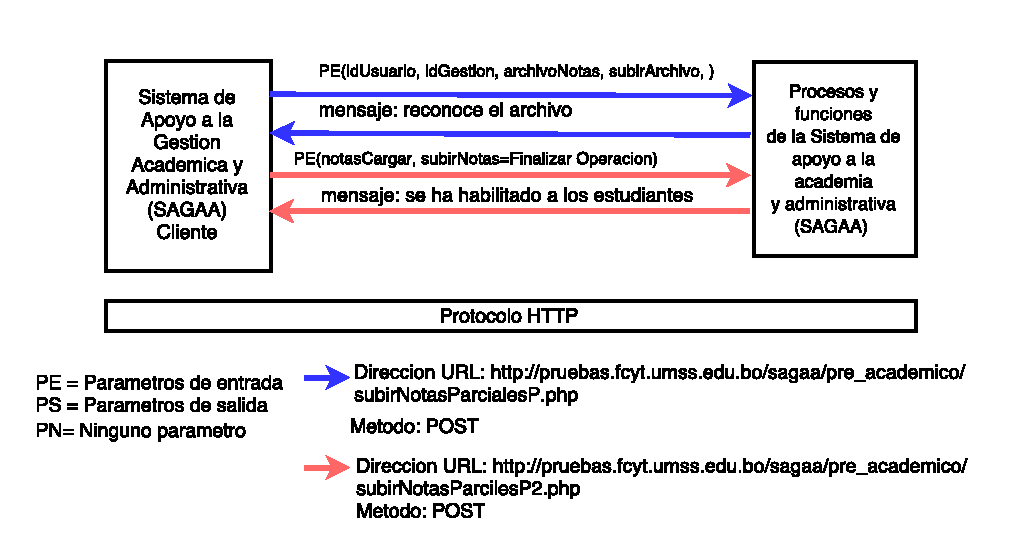
\includegraphics[width=0.4\textwidth]{disenoOperacionSubir.pdf}
\captionsetup{justification=centering, margin=2cm}
\caption{Dise'no de interfaz l'ogico para subir la planilla de nota, Fuente: Elaboraci'on propia}
\label{fig:DisenoSubir}
\end{figure}
En la \ref{fig:DisenoSubir} se ha representado la secuencia de peticiones de los m'etodos y par'ametros que se han utilizado para el desarrollo del \textsc{"servicio planilla de notas"}.

\subsection{Dise'no de mensajes}
Para el presente proyecto el \textsc{"servicio planilla de notas"}, el  dise'no de mensajes que env'ia y recibe, son definidos como los mensajes de entrada, salida y excepciones.

\begin{figure}
\centering
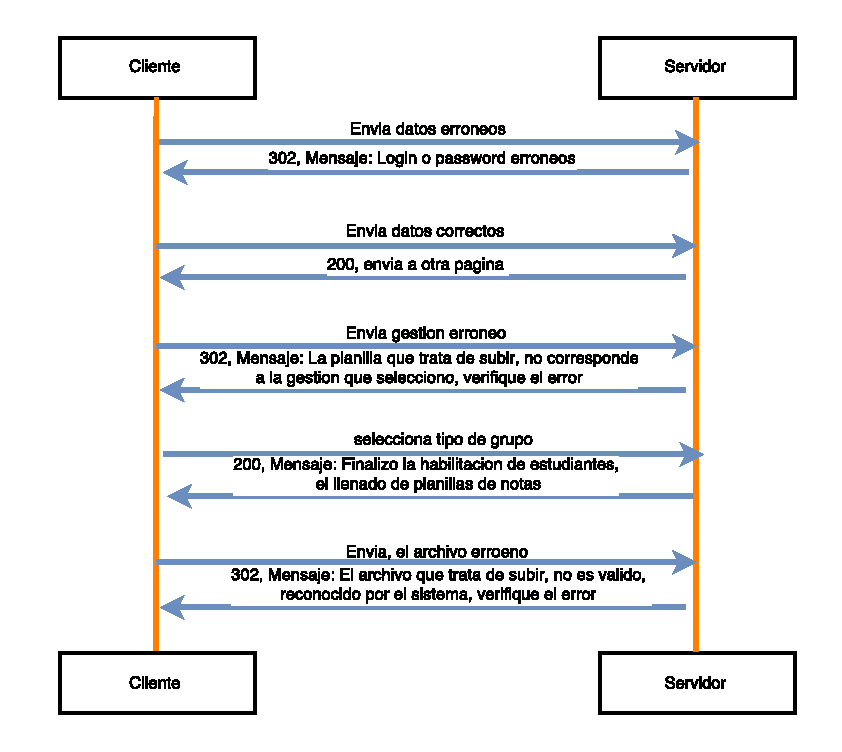
\includegraphics[width=0.4\textwidth]{disenoMensaje.pdf}
\captionsetup{justification=centering, margin=2cm}
\caption{Dise'no de mensaje de entradas, salidas y excepciones, Fuente: Elaboraci'on propia}
\label{fig:DisenoMensaje}
\end{figure}
En la \ref{fig:DisenoMensaje}, se ha representado la secuencia de peticiones, los mensajes que el SAGAA responde, que se han utilizado para el desarrollo del \textsc{"servicio planilla de notas"}.





